\documentclass[12pt,twoside]{report}

% some definitions for the title page
\newcommand{\reporttitle}{Session-Typed Programming with Nested Protocols in Go}
\newcommand{\reportauthor}{Benito Echarren Serrano}
\newcommand{\supervisor}{Prof. Nobuko Yoshida}
\newcommand{\secondmarker}{Dr. Iain Phillips}
\newcommand{\reporttype}{Final Report}
\newcommand{\degreetype}{MEng Computing} 

\newcommand{\comment}[1]{}
\newcommand{\white}{\ \ \ \ \ \ \ \ \ \ \ \ }
\newcommand{\pad}{\ \ \ \ \ \ }
% load some definitions and default packages
%%%%%%%%%%%%%%%%%%%%%%%%%%%%%%%%%%%%%%%%%
% University Assignment Title Page 
% LaTeX Template
% Version 1.0 (27/12/12)
%
% This template has been downloaded from:
% http://www.LaTeXTemplates.com
%
% Original author:
% WikiBooks (http://en.wikibooks.org/wiki/LaTeX/Title_Creation)
%
% License:
% CC BY-NC-SA 3.0 (http://creativecommons.org/licenses/by-nc-sa/3.0/)
% 
%
%%%%%%%%%%%%%%%%%%%%%%%%%%%%%%%%%%%%%%%%%
%----------------------------------------------------------------------------------------
%	PACKAGES AND OTHER DOCUMENT CONFIGURATIONS
%----------------------------------------------------------------------------------------
\usepackage[a4paper,hmargin=2.8cm,vmargin=2.0cm,includeheadfoot]{geometry}
\usepackage{textpos}
\usepackage[numbers]{natbib} % for bibliography
\usepackage{tabularx,longtable,multirow,subfigure,caption}%hangcaption
\usepackage{fncylab} %formatting of labels
\usepackage{fancyhdr} % page layout
\usepackage{url} % URLs
\usepackage[english]{babel}
\usepackage{amsmath}
\usepackage{graphicx}
\usepackage{dsfont}
\usepackage{epstopdf} % automatically replace .eps with .pdf in graphics
% \usepackage{backref} % needed for citations
\usepackage{array}
\usepackage{latexsym}
\usepackage{semantic}
\usepackage{xfrac}
\usepackage{fourier}
\usepackage{ amssymb }


\usepackage{listings}
\usepackage{color}


\lstset{frame=tb,
  language=Java,
  aboveskip=3mm,
  belowskip=3mm,
  showstringspaces=false,
  columns=flexible,
  basicstyle={\ttfamily},
  numbers=left,
  numberstyle=\tiny\color{gray},
  keywordstyle=\color{blue},
  commentstyle=\color{dkgreen},
  stringstyle=\color{mauve},
  breaklines=true,
  breakatwhitespace=true,
  tabsize=3,
  frame=single,
}
\definecolor{dkgreen}{rgb}{0,0.6,0}
\definecolor{gray}{rgb}{0.5,0.5,0.5}
\definecolor{mauve}{rgb}{0.58,0,0.82}
\definecolor{granate}{rgb}{0.68, 0.02, 0.55}

\lstdefinelanguage{Scribble}{
  keywords={global, protocol, rec, role, choice, at, continue, do, from, to, var, if, in, while, do, else, case, break, calls, new, nested, accept, invite, create},
  keywordstyle=\color{granate}\bfseries,
  ndkeywords={class, export, boolean, throw, implements, import, this},
  ndkeywordstyle=\color{darkgray}\bfseries,
  identifierstyle=\color{black},
  sensitive=false,
  comment=[l]{//},
  morecomment=[s]{/*}{*/},
  commentstyle=\color{dkgreen}\ttfamily,
  stringstyle=\color{dkgreen}\ttfamily,
  morestring=[b]',
  morestring=[b]"
}


% \usepackage[pdftex,pagebackref,hypertexnames=false,colorlinks]{hyperref} % provide links in pdf
\usepackage[pdftex,hypertexnames=false,colorlinks]{hyperref} % provide links in pdf

\hypersetup{pdftitle={},
  pdfsubject={}, 
  pdfauthor={},
  pdfkeywords={}, 
  pdfstartview=FitH,
  pdfpagemode={UseOutlines},% None, FullScreen, UseOutlines
  bookmarksnumbered=true, bookmarksopen=true, colorlinks,
    citecolor=black,%
    filecolor=black,%
    linkcolor=black,%
    urlcolor=black}

\usepackage[all]{hypcap}

% {} limita scope de color
% \newcommand{\global}{{\color{blue}\mathtt{global}}}

%\usepackage{color}
%\usepackage[tight,ugly]{units}
%\usepackage{float}
%\usepackage{tcolorbox}
%\usepackage[colorinlistoftodos]{todonotes}
% \usepackage{ntheorem}
% \theoremstyle{break}
% \newtheorem{lemma}{Lemma}
% \newtheorem{theorem}{Theorem}
% \newtheorem{remark}{Remark}
% \newtheorem{definition}{Definition}
% \newtheorem{proof}{Proof}


%%% Default fonts
\renewcommand*{\rmdefault}{bch}
\renewcommand*{\ttdefault}{cmtt}



%%% Default settings (page layout)
\setlength{\parindent}{0em}  % indentation of paragraph

\setlength{\parindent}{0em}  % indentation of paragraph

\setlength{\headheight}{14.5pt}
\pagestyle{fancy}
\renewcommand{\chaptermark}[1]{\markboth{\chaptername\ \thechapter.\ #1}{}} 
%\fancyhead[RO]{\sffamily \textbf{\thepage}} %Page no.in the right on even pages
%\fancyhead[LE]{\sffamily \textbf{\thepage}} %Page no. in the left on odd pages

\fancyfoot[ER,OL]{\thepage}%Page no. in the left on
                                %odd pages and on right on even pages
\fancyfoot[OC,EC]{\sffamily }
\renewcommand{\headrulewidth}{0.1pt}
\renewcommand{\footrulewidth}{0.1pt}
% \captionsetup{margin=10pt,font=small,labelfont=bf}
\captionsetup{margin=10pt,font=small}

%--- chapter heading

\def\@makechapterhead#1{%
  \vspace*{10\p@}%
  {\parindent \z@ \raggedright \sffamily
    \interlinepenalty\@M
    \Huge\bfseries \thechapter \space\space #1\par\nobreak
    \vskip 30\p@
  }}

%--- chapter heading

\def\@makechapterhead#1{%
  \vspace*{10\p@}%
  {\parindent \z@ \raggedright \sffamily
        %{\Large \MakeUppercase{\@chapapp} \space \thechapter}
        %\\
        %\hrulefill
        %\par\nobreak
        %\vskip 10\p@
    \interlinepenalty\@M
    \Huge\bfseries \thechapter \space\space #1\par\nobreak
    \vskip 30\p@
  }}

%---chapter heading for \chapter*  
\def\@makeschapterhead#1{%
  \vspace*{10\p@}%
  {\parindent \z@ \raggedright
    \sffamily
    \interlinepenalty\@M
    \Huge \bfseries  #1\par\nobreak
    \vskip 30\p@
  }}	
\allowdisplaybreaks

% load some macros
% Here, you can define your own macros. Some examples are given below.

\newcommand{\R}[0]{\mathds{R}} % real numbers
\newcommand{\Z}[0]{\mathds{Z}} % integers
\newcommand{\N}[0]{\mathds{N}} % natural numbers
\newcommand{\C}[0]{\mathds{C}} % complex numbers
\renewcommand{\vec}[1]{{\boldsymbol{{#1}}}} % vector
\newcommand{\mat}[1]{{\boldsymbol{{#1}}}} % matrix


% {} limita scope de color
% Scribble syntax macros
\newcommand{\scrglobal}{{\color{blue}\mathtt{global}}}
\newcommand{\nested}{{\color{blue}\mathtt{nested}}}
\newcommand{\protocol}{{\color{blue}\mathtt{protocol}}}
\newcommand{\scrlocal}{{\color{blue}\mathtt{local}}}
\newcommand{\role}{{\color{blue}\mathtt{role}}}
\newcommand{\choice}{{\color{blue}\mathtt{choice}}}
\newcommand{\scrdo}{{\color{blue}\mathtt{do}}}
\newcommand{\rec}{{\color{blue}\mathtt{rec}}}
\newcommand{\calls}{{\color{blue}\mathtt{calls}}}
\newcommand{\continue}{{\color{blue}\mathtt{continue}}}
\newcommand{\from}{{\color{blue}\mathtt{from}}}
\newcommand{\scrto}{{\color{blue}\mathtt{to}}}
\newcommand{\scrend}{{\color{blue}\mathtt{end}}}
\newcommand{\scrnew}{{\color{blue}\mathtt{new}}}
\newcommand{\at}{{\color{blue}\mathtt{at}}}
\newcommand{\scror}{{\color{blue}\mathtt{or}}}
\newcommand{\invite}{{\color{blue}\mathtt{invite}}}
\newcommand{\create}{{\color{blue}\mathtt{create}}}
\newcommand{\scrin}{{\color{blue}\mathtt{in}}}
\newcommand{\accept}{{\color{blue}\mathtt{accept}}}

\newcommand{\project}{\projectenv{Env}}
\newcommand{\projectenv}[1]{\downarrow_A^{#1}}
\newcommand{\roles}[2]{\mathit{#1_1},\ ...\ ,\ \mathit{#1_#2}}
\newcommand{\rolessig}[2]{\role\ \mathit{#1_1},\ ...\ ,\ \role\ \mathit{#1_#2}}
\newcommand{\scrmessage}[2]{\mathtt{#1}(\mathtt{#2})}
\newcommand{\varinset}[2]{{#1 \in #2}}

\newcommand{\choiceG}[4]{\choice\ \at\ \mathit{#1}\ \{\,\mathit{#2}_{#3}\,\}_{\varinset{#3}{#4}}}
\newcommand{\messageG}[4]{\scrmessage{#1}{#2}\ \from\ \mathit{#3}\ \scrto\ \mathit{#4}}
\newcommand{\recG}[2]{\rec\ \mathit{#1}\ \{\,\mathit{#2}\,\}}
\newcommand{\continueG}[1]{\continue\ \mathit{#1}}
\newcommand{\callsG}[3]{\mathit{#1}\ \calls\ \mathit{#2}(\roles{#3}{n})}
\newcommand{\doG}[2]{\scrdo\ \mathit{#1}(\roles{#2}{n})}
\newcommand{\contG}[2]{#1;\ \mathit{#2}}

\newcommand{\choiceL}[4]{\choice\ \at\ \mathit{#1}\ \{\,\mathit{#2}_{#3}\,\}_{\varinset{#3}{#4}}}
\newcommand{\messageFromL}[3]{\scrmessage{#1}{#2}\ \from\ \mathit{#3}}
\newcommand{\messageToL}[3]{\scrmessage{#1}{#2}\ \scrto\ \mathit{#3}}
\newcommand{\recL}[2]{\rec\ \mathit{#1}\ \{\,\mathit{#2}\,\}}
\newcommand{\continueL}[1]{\continue\ \mathit{#1}}
\newcommand{\inviteL}[2]{\invite(\roles{#1}{n})\ \scrto\ \mathit{#2}}
\newcommand{\createL}[2]{\create(\rolessig{#1}{m})\ \scrin\ \mathit{#2}}
\newcommand{\acceptL}[4]{\accept\ \mathit{#1}(\roles{#2}{n};\ \scrnew\ \roles{#3}{m})\ \from\ \mathit{#4}}
\lstset{frame=tb,
  language=Java,
  aboveskip=3mm,
  belowskip=3mm,
  showstringspaces=false,
  columns=flexible,
  basicstyle={\ttfamily},
  numbers=left,
  numberstyle=\tiny\color{gray},
  keywordstyle=\color{blue},
  commentstyle=\color{dkgreen},
  stringstyle=\color{mauve},
  breaklines=true,
  breakatwhitespace=true,
  tabsize=3,
  frame=single,
}
\definecolor{dkgreen}{rgb}{0.078, 0.580, 0.086}
\definecolor{gray}{rgb}{0.5,0.5,0.5}
\definecolor{mauve}{rgb}{0.58,0,0.82}
\definecolor{granate}{rgb}{0.68, 0.02, 0.55}

\lstdefinelanguage{Scribble}{
  keywords={global, protocol, rec, role, choice, at, continue, do, from, to, var, if, in, while, do, else, case, break, calls, new, nested, accept, invite, create, local},
  keywordstyle=\color{blue}\bfseries,
  ndkeywords={class, export, boolean, throw, implements, import, this},
  ndkeywordstyle=\color{mauve}\bfseries,
  identifierstyle=\color{black},
  sensitive=false,
  comment=[l]{//},
  morecomment=[s]{/*}{*/},
  commentstyle=\color{dkgreen}\ttfamily,
  stringstyle=\color{dkgreen}\ttfamily,
  morestring=[b]',
  morestring=[b]"
}

\lstdefinelanguage{Pseudocode}{
  keywords={end, global, protocol, rec, role, choice, at, continue, do, from, to, var, if, in, while, do, else, case, break, calls, new, nested, accept, invite, create, local},
  % keywordstyle=\color{granate}\bfseries,
  ndkeywords={def, match, with, for, class, return, export, boolean, throw, implements, import, this},
  ndkeywordstyle=\color{mauve}\bfseries,
  identifierstyle=\color{black},
  sensitive=false,
  comment=[l]{//},
  morecomment=[s]{/*}{*/},
  commentstyle=\color{dkgreen}\ttfamily,
  stringstyle=\color{dkgreen}\ttfamily,
  morestring=[b]',
  morestring=[b]"
}


% NOTATION
\definecolor{purple}{rgb}{0.415, 0.035, 0.827}
% \definecolor{dkorange}{rgb}{0.870, 0.427, 0.007}
\definecolor{dkorange}{rgb}{0.709, 0.482, 0.050}
\definecolor{dkpurple}{rgb}{0.227, 0.031, 0.631}
% \definecolor{dkred}{rgb}{0.878, 0.094, 0}
\definecolor{dkred}{rgb}{0.8, 0.019, 0}
% \definecolor{lightblue}{rgb}{0.047, 0.752, 0.811}
\definecolor{lightblue}{rgb}{0.043, 0.588, 0.6}
% \definecolor{dkyellow}{rgb}{0.678, 0.654, 0}
\definecolor{dkyellow}{rgb}{0.4, 0.4, 0.039}


% GO KWDS
\newcommand{\kwd}[1]{{\color{mauve} \texttt{#1}}}
\newcommand{\gotype}{\kwd{type}}
\newcommand{\gostruct}{\kwd{struct}}
\newcommand{\gointerface}{\kwd{interface}}
\newcommand{\gogo}{\kwd{go}}
\newcommand{\gofunc}{\kwd{func}}
\newcommand{\gochan}{\kwd{chan}}
\newcommand{\goconst}{\kwd{const}}
\newcommand{\goiota}{\kwd{iota}}
\newcommand{\godefer}{\kwd{defer}}
\newcommand{\gopanic}{\kwd{panic}}
% GO KWDS

% Reserved words
\newcommand{\protocolname}[1]{{\mathit{#1}}}
\newcommand{\rolename}[1]{{\mathit{#1}}}
\newcommand{\localprotocol}[2]{{#1@#2}}
\newcommand{\localprotocolname}[2]{{\mathit{#2}\_\mathit{#1}}}

% NOTATION
% Variables
\newcommand{\varname}[1]{{\mathtt{#1}}}

% Types
\newcommand{\typename}[1]{{\color{dkpurple}\mathtt{#1}}}

% Directory structure
\newcommand{\filename}[1]{{\color{dkgreen} \mathtt{#1.go}}}
\newcommand{\dirname}[1]{{\color{dkgreen} \mathtt{#1}/}}
\newcommand{\pkgname}[1]{{\color{dkgreen} \mathtt{#1}}}

% Structs
% \newcommand{\structname}[1]{{\color{dkred} \mathit{#1}}}
% \newcommand{\structfield}[1]{{\color{dkred} \mathtt{#1}}}

% Functions and Interfaces
% \newcommand{\functionname}[1]{{\color{dkyellow} \mathtt{#1}}}
% \newcommand{\interfacename}[1]{{\color{dkyellow} \mathit{#1}}}

% Structs
\newcommand{\structfield}[1]{{\color{dkred} \mathtt{#1}}}
\newcommand{\functionname}[1]{{\color{dkred} \mathit{#1}}}

% Functions and Interfaces
\newcommand{\structname}[1]{{\color{dkyellow} \mathtt{#1}}}
\newcommand{\interfacename}[1]{{\color{dkyellow} \mathit{#1}}}

% Enums
\newcommand{\enumtype}[1]{{\color{lightblue} \mathit{#1}}}
\newcommand{\enumvalue}[1]{{\color{lightblue} \mathtt{#1}}}

% NOTATION

% HELPER CMDS
\newcommand{\wg}{\varname{wg}}
\newcommand{\rolechannels}{\varname{roleChannels}}
\newcommand{\invitechannels}{\varname{inviteChannels}}
\newcommand{\envparam}{\varname{env}}
\newcommand{\payloaddecl}[3]{\structfield{#1_1}:\ \typename{#2_1},\ ...\ ,\ \structfield{#1_{#3}}:\ \typename{#2_{#3}}}
\newcommand{\pkgstructaccess}[2]{\pkgname{#1}.\structname{#2}}
\newcommand{\pkginterfaceaccess}[2]{\pkgname{#1}.\interfacename{#2}}
\newcommand{\pkgfuncaccess}[2]{\pkgname{#1}.\functionname{#2}}
\newcommand{\methodcall}[2]{\varname{#1}.\functionname{#2}}
\newcommand{\assignment}[2]{\varname{#1}\ :=\ #2}
\newcommand{\waitgroup}{\pkgstructaccess{sync}{WaitGroup}}
\newcommand{\rolechantype}[2]{\pkgstructaccess{#2\_channels}{#1\_Chan}}
\newcommand{\invitechantype}[2]{\pkgstructaccess{invitations}{\localprotocol{#1}{#2}\_InviteChan}}
\newcommand{\envtype}[2]{\pkgstructaccess{callbacks}{\localprotocol{#1}{#2}\_Env}}
\newcommand{\resulttype}[2]{\pkgstructaccess{#2\_results}{#1\_Result}}
\newcommand{\roleimplparams}{\wg,\ \rolechannels,\ \invitechannels,\ \envparam}
% HELPER CMDS

% load title page
\begin{document}
% Last modification: 2015-08-17 (Marc Deisenroth)
\begin{titlepage}

\newcommand{\HRule}{\rule{\linewidth}{0.5mm}} % Defines a new command for the horizontal lines, change thickness here

%----------------------------------------------------------------------------------------
%	LOGO SECTION
%----------------------------------------------------------------------------------------


\includegraphics[width = 4cm]{./figures/imperial}\\[0.5cm] 

\center % Center everything on the page
 
%----------------------------------------------------------------------------------------
%	HEADING SECTIONS
%----------------------------------------------------------------------------------------

\textsc{\LARGE \reporttype}\\[1.5cm] 
\textsc{\Large Department of Computing}\\[0.5cm] 
\textsc{\large Imperial College of Science, Technology and Medicine}\\[0.5cm] 

%----------------------------------------------------------------------------------------
%	TITLE SECTION
%----------------------------------------------------------------------------------------

\HRule \\[0.4cm]
{ \huge \bfseries \reporttitle}\\ % Title of your document
\HRule \\[1.5cm]
 
%----------------------------------------------------------------------------------------
%	AUTHOR SECTION
%----------------------------------------------------------------------------------------

\begin{minipage}{0.4\textwidth}
\begin{flushleft} \large
\emph{Author:}\\
\reportauthor % Your name
\end{flushleft}
\end{minipage}
~
\begin{minipage}{0.4\textwidth}
\begin{flushright} \large
\emph{Supervisor:} \\
\supervisor\\[5pt] % Supervisor's Name
\emph{Second Marker:}\\
\secondmarker
\end{flushright}
\end{minipage}\\[4cm]




%----------------------------------------------------------------------------------------


%----------------------------------------------------------------------------------------
%	DATE SECTION
%----------------------------------------------------------------------------------------

{\large \today} % Date, change the \today to a set date if you want to be precise


\vfill % Fill the rest of the page with whitespace
Submitted in partial fulfillment of the requirements for the \degreetype~of Imperial College London

\end{titlepage}

\setcitestyle{square}


% page numbering etc.
\pagenumbering{roman}
\clearpage{\pagestyle{empty}\cleardoublepage}
\setcounter{page}{1}
\pagestyle{fancy}

%%%%%%%%%%%%%%%%%%%%%%%%%%%%%%%%%%%%
% \begin{abstract}
% Your abstract.
% \end{abstract}

\cleardoublepage
%%%%%%%%%%%%%%%%%%%%%%%%%%%%%%%%%%%%
% \section*{Acknowledgments}
% Comment this out if not needed.

% \clearpage{\pagestyle{empty}\cleardoublepage}

%%%%%%%%%%%%%%%%%%%%%%%%%%%%%%%%%%%%
%--- table of contents
\fancyhead[RE,LO]{\sffamily {Table of Contents}}
\tableofcontents 


\clearpage{\pagestyle{empty}\cleardoublepage}
\pagenumbering{arabic}
\setcounter{page}{1}
\fancyhead[LE,RO]{\slshape \rightmark}
\fancyhead[LO,RE]{\slshape \leftmark}

%%%%%%%%%%%%%%%%%%%%%%%%%%%%%%%%%%%%
\chapter{Introduction}
From the multiple cores in a CPU or GPU to the large server clusters in data centers, concurrency and parallelism have become an inherent part of computers and how they are used. This distributed computation model gives much higher performance and scalability, as multiple tasks can be executed at the same time, but it also makes reasoning about the software much harder, giving rise to concurrency bugs such as race conditions and deadlocks.\\

In order to reason about these concurrent and parallel programs, researchers have come up with different memory models with different guarantees. The two most important ones are shared memory and message passing. Shared memory is an abstraction where all the components can read and write to a single piece of memory, and the changes that anyone makes become visible to the other participants. On the other hand, message passing expresses the communications between different components as a series of message exchanges, with each process having its own address space. %However reasoning about it can be tricky, as some compiler and hardware optimisations reorder the instructions, and when different threads read and write to the same location in memory, race conditions can occur.
\\

When writing a concurrent program, understanding the concurrency model that you are using is vital to writing correct code. However, unlike the type system which provides some correctness guarantees about the program at compile time (type safety of assignments, method calls, etc.), programming languages generally offer little to no support when it comes to statically detecting concurrency bugs (deadlocks, race conditions, etc.). Although separate tools for different programming languages have been developed to do this, like FindBugs\cite{FindBugs} or Jlint\cite{JLint} for Java\comment{How Good is Static Analysis at Finding Concurrency Bugs?/Find Bugs paper and chord paper}, they do not scale well with the size of the program and may not find all the concurrency bugs in the implementation\cite{ConcurrencyTools}. Session types\cite{binarysessiontypes1} provide an alternative approach for reasoning about inter-process communication in a message passing setting. They formalise the structured interactions between the participants as a protocol, ensuring that there are no communication errors or concurrency bugs in the program. Instead of trying to find bugs in an existing implementation, session types guarantee that the implementation will be free of concurrency bugs. Unlike data types, which express the type of information that will be stored in memory during execution, session types describe the communication exchanges between processes.\\

% On the other hand, in message passing the components communicate by exchanging data in the form of explicit messages. This model can be used to express the communication between different components in a distributed system. The interactions of different participants exchanging typed data following a protocol can be formalized using session types \comment{ref session types}, which guarantee that communication errors such as deadlocks or receiving unexpected messages will not happen.
Session types have been extended in different directions in order to be more expressive by providing more control over the interactions through means such as logical assertions\cite{logicaassertions}. The theory has also been extended to allow greater flexibility on how participants can join or leave a session\cite{multirolesessiontypes} or having a parametric number of participants acting a particular role (e.g. n workers)\cite{parametrictypes}.\\

However, modern protocols have grown and become more complex. Often, they will have a highly modular structure, with a protocol calling or depending on other protocols. Moreover, different protocols may also share some common structure, with interactions between different participants following the same pattern. For instance, a protocol where a client wants to communicate with a server might initially involve authenticating with a different authentication server in order to get a valid token. This set of interactions with the authentication server could be considered a different subprotocol, which might also be used by many different applications in their authentication process. \\

Demangeon et al.\cite{nestedprotocols} extended the existing session type theory in order to allow nesting of protocols using subsessions and invitations. This new theory allows structuring such protocols in a more intuitive way and even provides the ability to be able to reuse subprotocols for different use cases. They also allow multiple calls to the same protocol with potentially different parameters, making the protocols more concise and readable. Subprotocols can also invite new participants to participate in them, which allows defining protocols with a dynamic number of participants. We develop the first implementation of this theory to give a session type-based framework for the specification and safe implementation of distributed programs in Go.\\

Existing session type-based frameworks required the number of participants to fixed at the start of the session. However, in nested protocols participants can be introduced into the session dynamically. Go can handle this kind of task very well by using two of its in-built primitives for concurrency\cite{godocs}: the ability to spawn thousands of lightweight threads called \textit{goroutines} and \textit{channels}, which allow inter-process communication through message passing. Dynamically delegating tasks by spawning new goroutines is common practice in Go, so this programming model is highly suitable for implementing nested protocols.

%The toolchain generates an implementation of the different roles in the protocol, allowing the user to define logic through callbacks. 
% \begin{figure}[tb]
% \centering
% 
\includegraphics[width = 0.4\hsize]{./figures/imperial}
% \caption{Imperial College Logo. It is nice blue, and the font is quite stylish. But you can choose a different one if you do not like it.}
% \label{fig:logo}
% \end{figure}

% Figure~\ref{fig:logo} is an example of a figure. 

%%%%%%%%%%%%%%%%%%%%%%%%%%%%%%%%%%%%
\chapter{Background}

\section{Session Types}
\subsection{Overview}

The two main models to reason about concurrent programs are shared memory and message passing. In shared memory, components communicate by reading and writing to a shared part of memory. This is how CPU threads and processes in a computer communicate with each other. However, reasoning about concurrent programs with this model can be tricky, as compiler and hardware optimisations can reorder the program's instructions\cite{sharedmemory}. On the other hand, in message passing inter-process communication is carried out by exchanging data in the form of explicit messages. This model closely resembles how communication is carried out in distributed systems.\\

Message passing can be encoded using the $\pi$-calculus, a process algebra based on name passing which was developed by Milner\cite{milnerpicalc}. In this calculus, processes communicate by sending channel names over named channels. We present an asynchronous variant of the $\pi$-calculus in section \ref{pi-calculus}. Session types\cite{binarysessiontypes1} introduce a typing discipline for formalising the communication exchanges between processes in the $\pi$-calculus. The initial theory was defined only for two participants, but it was later extended by Honda et al.\cite{asyncmpst1, asyncmpst2} to include multiple parties. This allowed the session types to encode a larger number of protocols. Session types improve the reliability of distributed systems by guaranteeing the correctness of the programs. If the processes are well-typed, they will have session fidelity and will not suffer from communication errors such as deadlocks, type mismatches or protocol violations.\\

There are already multiple implementations of session types for popular programming languages such as Java\cite{java}, C\cite{mpstc}, Go\cite{parametrictypes}, Python\cite{python}, Erlang\cite{erlang}, etc. Due to the set of features available to different programming languages, the implementation of MPST varies from one language to another. Some languages use rely on the type system to verify the correctness of the session's implementation at compile-time, while others may require run-time checks in order to detect protocol violations. 

\subsection{Asynchronous $\pi$-Calculus}\label{pi-calculus}
The $\pi$-calculus is a process algebra for encoding communicating systems. Processes communicate with one another through name passing, by sending and receiving channel names over named channels. The $\pi$-calculus is a simple yet powerful model which has been shown to be Turing-complete\cite{turingcomplete}, as it can encode the $\lambda$-calculus. The original theory was proposed by Robin Milner\cite{milnerpicalc}, but different variants have been proposed since. The first asynchronous $\pi$-calculus theory was presented in \cite{asyncandpicalc}, and we present a variant based on this theory, as defined in \cite{co406}.

\begin{figure}[h]
    \centering
    \begin{equation*}
    \centering
    \begin{array}{rrlcr}
        P,\ Q & ::= && \white & Processes \\[2.75pt]
             &   & 0 & \white & Nil\ Process  \\[2.75pt]
             & | & P\ |\ Q & \white & Parallel\ Composition \\[2.75pt]
             & | & (\nu\ a)\ P & \white & Scope Restriction \\[2.75pt]
             & | & !P & \white  & Replication \\[2.75pt]
             & | & \overline{u}\langle v \rangle & \white & Output \\[2.75pt] 
             & | & u(x).P & \white & Input \\\\
        u,\ v & ::= && \white & Identifiers \\[2.75pt]
              &   & a,\ b,\ c & \white & Names \\[2.75pt]
              & | & x,\ y,\ z & \white & Variables \\
        \end{array}
    \end{equation*}
    \caption{Syntax of monadic asynchronous  $\pi$-calculus}
    \label{picalc_syntax}
\end{figure}{}

The syntax of the asynchronous $\pi$-calculus is defined in Figure \ref{picalc_syntax}:
\begin{itemize}
    \item $0$ is the nil process, which represents the process with no actions.
    \item $P\ |\ Q$ is the parallel composition of two processes. These processes can execute in any order.
    \item $(\nu\ a)\ P$ is the scope restriction operation. It creates a new named channel $a$ that can only be used within process P and will not interfere with any other existing names.
    \item $!P$ is process replication. It represents the infinite parallel composition of process $P$: $P\ |\ P\ |\ P\ |\ ...$
    \item $\overline{u}\langle v \rangle$ is the output operation, which sends $v$ over $u$.
    \item $u(x).P$ is the input operation. It receives a a value over channel $u$. After receiving the value  it will continue executing process P, replacing all references to $x$ in $P$ with the received value.
\end{itemize}

Structural congruence is an equivalence relation which expresses that two processes are equivalent/interchangeable. We define the structural congruence of asynchronous $\pi$-calculus relation in Figure \ref{picalc_cong}.\\

\begin{figure}[h]
    \centering
    \begin{equation*}
    \centering
    \begin{array}{rcrclcr}
         & & P & \equiv & P & & Reflexivity\\[2.75pt]
         P \equiv Q & \implies & Q &\equiv\ & P & & Symmetry  \\[2.75pt]
         P \equiv Q\ \land\ Q \equiv R & \implies & P & \equiv & R & & Transitivity \\[2.75pt]
         P \equiv Q\ & \implies & (\nu\ a)\ P & \equiv & (\nu\ a)\ Q & & Cong\ of\ Restriction \\[2.75pt]
         P \equiv Q\ & \implies & P\ |\ R & \equiv & Q\ |\ R & & Cong\ of\ Parallel\ Comp \\[2.75pt]
         P \equiv Q & \implies & u(x).P & \equiv & u(x).Q & & Cong\ of\ Input \\[2.75pt]
         P \equiv Q & \implies & !P & \equiv & !Q & & Cong\ of\ Replication \\[2.75pt]
         P\ =_\alpha \ Q\ & \implies & P & \equiv & Q &  & \alpha-equivalence \\[2.75pt]
         & & P\ |\ (Q\ |\ R) & \equiv & (P\ |\ Q)\ |\ R & & Associativity \\[2.75pt]
         & & P\ |\ Q & \equiv & Q\ |\ P & & Commutativity \\[2.75pt]
         & & P\ |\ 0 & \equiv & P & & Zero \\[2.75pt]
         & & !P & \equiv & P\ |\ !P & & Replication \\[2.75pt]
         & & (\nu\ a)\ 0 & \equiv & 0 & & Res\ of\ Nil \\[2.75pt]
         & & (\nu\ a)(\nu\ b)\ P\ & \equiv & (\nu\ b)(\nu\ a)\ P & & Res\ of\ Restriction \\[2.75pt]
         a\ \notin\ fn(P) & \implies & \ P\ |\ (\nu\ a)\ Q & \equiv & (\nu\ a)(P\ |\ Q) & & Res\ over\ Parallel\ Comp
        \end{array}
    \end{equation*}
    \caption{Structural congruence of monadic asynchronous  $\pi$-calculus}
    \label{picalc_cong}
\end{figure}{}

The operational semantics of the $\pi$-calculus shown in Figure \ref{picalc_op_sem} define how the communication between the processes happens. The most important rule is \textsc{Comm}, which shows how the value sent by the output process is received by the input process and used in its continuation $P$ by replacing the references to the variable $x$ in $P$.

\begin{figure}[h!]
    \centering
    \begin{equation*}
    \centering
    \begin{array}{c}
    \inference{}{\overline{a}\langle v \rangle\ |\ a(x).P\ \longrightarrow\ P\{\sfrac{v}{x}\}}[\textsc{Comm}]\\[20pt]
    \inference{P\ \longrightarrow\ P'}{P\ |\ Q\ \longrightarrow\ P'\ |\ Q}[\textsc{Par}]\\[20pt]
    \inference{P\ \longrightarrow\ P'}{(\nu\ a)\ P \longrightarrow\ (\nu\ a)\ P'}[\textsc{Res}]\\[20pt]
    \inference{
        P \equiv Q 
        & Q\ \longrightarrow\ Q' 
        & Q' \equiv P'
    }{P\ \longrightarrow\ P'}[\textsc{Struct}]
    \end{array}
    \end{equation*}
    \caption{Operational semantics of monadic asynchronous $\pi$-calculus}
    \label{picalc_op_sem}
\end{figure}{}

It is important to notice that the output process $\bar{u} \langle v \rangle$ does not have any continuation. This reflects the asynchronous nature of the calculus. However, the asynchronous pi calculus presented above is very expressive; it is possible to encode other variants of $\pi$-calculus using it, including synchronous $\pi$-calculus, which allows continuation after output, and polyadic $\pi$-calculus, which allows exchanging vectors of messages at once. 

% The intuition for encoding synchronous $\pi$-calculus is to use two additional channels to agree on a rendez-vous between the sender and the receiver. The sender will send a channel over which to communicate, and the receiver will send a private channel over which the exchange will actually take place. To encode polyadic synchronous $\pi$-calculus using monadic synchronous pi cal, 

% \begin{table}[]
%     \centering
%     \begin{tabular}{l|p{6cm}|p{6cm}}
%          &$monadic\ asynchronous\ \longrightarrow\ monadic \ synchronous$ & $mondadic\ synchronous\ \longrightarrow\ polyadic\ synchronous$ \\
%          \hline
%          \textsc{Input} & $\llbracket \bar{u} \langle v \rangle.P$\rrbracket = \hfill (\nu\ c)(\bar{u} \langle c \rangle\ |\ c(y).(\bar{y} \langle v\rangle\ |\ \llbracket P \rrbracket))& $\llbracket \bar{u} \langle v \rangle.P$\rrbracket = \hfill (\nu\ c)(\bar{u} \langle c \rangle\ |\ c(y).(\bar{y} \langle v\rangle\ |\ \llbracket P \rrbracket))
         
%     \end{tabular}
%     \caption{Caption}
%     \label{tab:my_label}
% \end{table}{}

\subsection{Binary Session Types}
A session is a unit of conversation between participants. Session types provide a structured way to define and reason about the communications which take place between participants. In binary session types, these interactions happen between two participants. A session results from the binary composition of the processes of each participant. There are multiple similar formulations for session types in the literature, but Figure \ref{bst_session_calc} shows the syntax for processes in binary session types as presented in \cite{co406}. %presented in \textit{the CO406 course}\comment{replace with reference}.\\

\begin{figure}[h]
    \centering
    \begin{equation*}
    \centering
    \begin{array}{rrlcr}
        v & ::= & \underline{n} & \white & Integers \\[2.75pt]
              & |  & \texttt{true}\ |\ \texttt{false} & \white & Booleans \\[2.75pt]
              & | & \texttt{"str"} & \white & Strings \\\\
        e,\ e' & ::= & v & \white & Values \\[2.75pt]
              & |  & x & \white & Variables \\[2.75pt]
              & | & e\ +\ e'\ |\ e\ -\ e'\ |\ -e & \white & Arithmetic \\[2.75pt]
              & | & e\ =\ e'\ |\ e\ <\ e'\ |\ e\ >\ e' & \white & Relational \\[2.75pt]
              & | & e\ \land\ e'\ |\ e\ \lor\ e'\ |\ \lnot e & \white & Logical \\
              & | & e\ \bigoplus\ e' & \white & Non-determinism\\\\
        
        
        p & ::= & Alice\ |\ Bob & \white & Participant\\\\
        P,\ Q & ::= && \white & Processes \\[2.75pt]
             &   & 0 & \white & Nil\ Process  \\[2.75pt]
             & | & \overline{p} \langle e \rangle.P & \white & Output \\[2.75pt] 
             & | & p(x).P & \white & Input\\[2.75pt]
             & | & p\ \triangleright\ \{l_i:\ P_i\}_{i\in I}& \white & Branching\\[2.75pt]
             & | & p\ \triangleleft\ l.P& \white & Selection \\[2.75pt]
             & | & \texttt{if}\ e\ \texttt{then}\ P\ \texttt{else}\ Q & \white & Conditional \\[2.75pt]
             & | & \mu X.P & \white  & Recursive\ Process \\[2.75pt]
             & | & X & \white  & Recursive\ Variable \\\\
             
        M & ::= & p :: P\ |\ q :: Q & \white & Binary\ Composition
        \end{array}
    \end{equation*}
    \caption{Processes in the binary session calculus}
    \label{bst_session_calc}
\end{figure}{}

\begin{itemize}
    \item $0$ is the nil process, which represents no actions.
    \item $\overline{p} \langle e \rangle.P$ is the output operation, which sends the value $e$ to participant $p$ with continuation $P$ (the session calculus is synchronous).
    \item $p(x).P$ is the input operation, which waits for participant $p$ to send a value $x$. Upon receiving the value, execution continues with $P$, with the received value replacing the references to $x$ in $P$.
    
    \item $p\ \triangleright\ \{l_i:\ P_i\}_{i\in I}$ is the branching operation. The process waits for participant $p$ to send a label $l\ =\ l_i$, for some $i \in I$. After receiving the label, execution continues with process $P_i$.
    
    \item $p\ \triangleleft\ l.P$ is the selection operation. The process sends label $l$ to participant $p$, then continues executing $P$.
    
    \item $\texttt{if}\ e\ \texttt{then}\ P\ \texttt{else}\ Q$ is the conditional operation. Expression $e$ should evaluate to a boolean. If $e$ evaluates to true then process $P$ is executed, otherwise, $Q$ is executed.
    
    \item $\mu X.P$ and $X$ are used to express recursion in the processes. The recursive process $\mu X.P \equiv P\{\sfrac{\mu X.P}{X}\}$, that is, you are able to replace all the instances of the recursion variable $X$ in P with $\mu X.P$. This allows you to carry out potentially infinite unfoldings of the process.
    
    \item $e\ \bigoplus\ e'$ expresses a non-deterministic choice between two expressions of the same type, so the expression could evaluate to the result of either of the two expressions. 
    
    \item The evaluation of expressions is only defined when the types match: logical expressions are only defined on expressions which evaluate to booleans, arithmetic expressions and $e\ <\ e'$ and $e\ >\ e'$ are only defined on integer values, and $e\ =\ e'$ is only defined if $e$ and $e'$ have the same type.
\end{itemize}{}

This session calculus is based on the $\pi$-calculus, so we can observe a great amount of similarities between the constructs in both calculi. The main differences are the introduction of the branching and selection operations (which can be encoded in the $\pi$-calculus), the definition of recursion and the conditional process. \\

% The operational semantics for a session $M\ =\ p::P\ |\ q::Q$ are defined in a similar manner to the $\pi$-calculus. Additional rules are required for the branching/selection and the conditional processes. Reducing a recursive process may involve unfolding the recursion multiple times through structural congruence. For a formal definition please\\

We introduce the definition of the session types in Figure \ref{bst_session_types}. We will not give the formal typing judgements for the processes, these can be found in \cite{co406, binarysessiontypes1, subtyping}\comment{Course material ref and possibly language primitives}. However, we give an intuition behind the correspondence between processes and their session types:

\begin{figure}[h]
    \centering
    \begin{equation*}
    \centering
    \begin{array}{rrlcr}
        S & ::= && \white & Session\ Type \\[2.75pt]
             &   & \texttt{end} & \white & Termination  \\[2.75pt]
             & | & p![U];\ S & \white & Value\ Send \\[2.75pt]
             & | & p?[U];\ S & \white & Value\ Receive \\[2.75pt]
             & | & p \bigoplus \{l_i\ :\ S_i\}_{i \in I} & \white& Selection \\[2.75pt]
             & | & p \& \{l_i\ :\ S_i\}_{i \in I} & \white & Branching \\[2.75pt] 
             & | & t & \white & Type\ Variable \\[2.75pt]
             & | & \mu t.S & \white & Recursive\ Type\\\\
        U & ::= & \texttt{int}\ |\ \texttt{bool}\ |\ \texttt{string}& \white & Sorts\ for\ Expressions
        \end{array}
    \end{equation*}
    \caption{Syntax of binary session types}
    \label{bst_session_types}
\end{figure}{}

\begin{itemize}
    \item $Bob(x).\overline{Bob} \langle x + 1 \rangle.0:\ Bob?[\texttt{int}];\ Bob![\texttt{int}];\ \texttt{end}$ - In order to infer the sort of the input variable it may be necessary to see how it is used in the process.
    \item $Alice\ \triangleleft\ choice.\overline{Alice} \langle \texttt{"hello"} \rangle.0:\ Alice \bigoplus \{choice:\ Alice![\texttt{str}];\ \texttt{end}\}$ - similarly for branching.
    \item In order to be able to specify a type for a conditional process $\texttt{if}\ e\ \texttt{then}\ P\ \texttt{else}\ Q$, both branches $P$ and $Q$ must have the same type $S$, and therefore the type of the conditional process will also $S$.
    \item $\mu t.S$ and $t$ are used to specify recursive types. They work much in the same way as recursive processes; recursive types can also unfolded by replacing instances of $t$ in $S$ by $\mu t.S$.
\end{itemize} 

\begin{figure}[h!]
    \centering
    \begin{equation*}
    \centering
    \begin{array}{rcl}
             \overline{\texttt{end}} & = & \texttt{end}  \\[2.75pt]
             \overline{p![U];\ S} & = & p?[U];\ \overline{S} \\[2.75pt]
             \overline{p?[U];\ S} & = & p![U];\ \overline{S} \\[2.75pt]
             \overline{p \bigoplus \{l_i\ :\ S_i\}_{i \in I}} & = & p \& \{l_i\ :\ \overline{S_i}\}_{i \in I}\\[2.75pt]
             \overline{p \& \{l_i\ :\ S_i\}_{i \in I}} & = & p \bigoplus \{l_i\ :\ \overline{S_i}\}_{i \in I}\\[2.75pt]
             \overline{\mu t.S} & = & \mu t.\overline{S}\\[2.75pt]
             \overline{t} & = & t
        \end{array}
    \end{equation*}
    \caption{Duality of binary session types}
    \label{bst_duality}
\end{figure}{}

A key concept in binary session types is duality. When two processes are composed in a session, in order for the session to progress correctly, both processes must be carrying out complimentary operations. For instance, if $Alice$ is trying to send a string to $Bob$, $Bob$ must be waiting to receive a string from $Alice$, otherwise the protocol is stuck. Similarly, if $Bob$ is waiting for a label from $Alice$ to decide which branch to execute, $Alice$'s process must send one of the expected labels. Not only must the constructs be complimentary, but the types of the messages being sent must also match. Therefore, in order for a session to be correct, the processes involved must be duals of one another. This will ensure that the binary session will always make progress and that the session continues to be well-typed as the protocol is carried out. The duality of binary session types is shown in Figure \ref{bst_duality}.



\subsection{Multiparty Session Types}
Binary session types have limited applications to real-world problems, as standard protocols tend to be much more complex and involve more than two participants. These interactions cannot always be correctly expressed as the composition of binary sessions between different pairs of participants. \\

Multiparty session types\cite{asyncmpst2} extend the theory by allowing protocols to have multiple participants, thus overcoming these limitations. The main idea is to introduce global types, which describe the multiparty interactions within a protocol from a global perspective, as well as deriving a specification of the behaviour of each participant as local session type through the projection operation. \\

There are multiple variants of processes and their respective MPST in the literature. We present the syntax for synchronous multiparty session types defined in \cite{verygentleintrotompst} in Figure \ref{MPST_processes}.

\begin{figure}[h]
    \centering
    \begin{equation*}
    \centering
    \begin{array}{rrlcr}
        P,\ Q & ::= && \white & Processes \\[2.75pt]
             &   & 0 & \white & Nil\ Process  \\[2.75pt]
             
             & | & \texttt{if}\ e\ \texttt{then}\ P\ \texttt{else}\ Q & \white & Conditional \\[2.75pt]
             & | & \mu X.P & \white  & Recursive\ Process \\[2.75pt]
             & | & X & \white  & Recursive\ Variable\\[2.75pt]
             & | & p!l \langle e \rangle.P & \white & Output \\[2.75pt]
             & | & \sum\limits_{i \in I} p?l_i(x_i).P_i & \white & Branching \\\\

        M & ::= &&& Multiparty\ Session\\[2.75pt]
        & | & p :: P\ & \white & Process\\[2.75pt]
        & | & M\ |\ M\ & \white & Parallel\ Composition\\\\
        
        &&p,\ q,\ r,\ ... & \white & Participants\\[2.75pt]
        &&e,\ e',\ ... & \white & Expressions\\[2.75pt]
        &&x,\ y,\ z,\ ... & \white & Expression\  variables
        \end{array}
    \end{equation*}
    \caption{Processes in multiparty session calculus}
    \label{MPST_processes}
\end{figure}{}

Although the syntax varies slightly from the one showed in Figure \ref{bst_session_calc}, the semantics are essentially the same. The main difference is that processes now send/receive a label with the value they communicate. Because sessions now involve multiple participants, it is necessary to specify the other participant for the exchange (it would have been possible to omit this information in binary session types). \\

In multiparty session types, when deriving the types for protocols we consider both the global type, which formally specifies the interactions between all the participants in the protocol from a global perspective and local session types, which characterize the interactions that each of the participants carry out within the global protocol. The parallel composition of processes satisfying the session types implements the behaviour of the global type. In this way, the implementations of the different participants are decoupled from one another, so they could be implemented separately and the overall implementation would be correct as long as they all follow their respective session types.

\begin{figure}[h]
    \centering
    \begin{equation*}
    \centering
    \begin{array}{rrlcr}
        S & ::= & \texttt{int}\ |\ \texttt{bool}\ |\ \texttt{string}& \white & Sorts\\\\
        \textsc{Global\ Types} & && &\\[3pt]
        G & ::= & \texttt{end} & \white & Termination  \\[2.75pt]
             & | & p \longrightarrow q: \{l_i( S_i).G_i\}_{i \in I} & \white & Branching \\[2.75pt] 
             & | & t & \white & Type\ Variable \\[2.75pt]
             & | & \mu t.G & \white & Recursive\ Type\\\\
             
        \textsc{Local Types} &&&& \\[3pt]
        T & ::= & \texttt{end} & \white & Termination  \\[2.75pt]
          & | & \bigoplus_{i \in I}\ p!l_i(S_i).T_i & \white& Selection \\[2.75pt]
          & | & \&_{i \in I}\ p?l_i(S_i).T_i & \white & Branching \\[2.75pt] 
          & | & t & \white & Type\ Variable \\[2.75pt]
          & | & \mu t.S & \white & Recursive\ Type
        
        \end{array}
    \end{equation*}
    \caption{Syntax of multiparty session types}
    \label{MPST_types}
\end{figure}{}

We present the syntax for global and local types in Figure \ref{MPST_types}. Similarly to the syntax of processes, the local session types are almost the same as the binary session types. Global types introduce a single construct for branching/selection, $p \longrightarrow q:\{l_i(S_i).G_i\}_{i \in I}$, in which participant $p$ sends to $q$ the label (and corresponding value) which will determine what the continuation is.\\

Each participant in the protocol enacts a role in the global type. The session type for each role is derived by projecting the global type onto that role, which essentially ignores all the interactions in which the role does not take part, leaving only the behaviour that needs to be implemented for that role within the protocol. The projection operation is defined in Figure \ref{MPST_projection}.\\

\begin{figure}[h]
    \centering
    \begin{equation*}
    \centering
    \begin{array}{rcl}
        
        (p \longrightarrow p':\{l_i(S_i).G_i\}_{i \in I}) \upharpoonright q & = &
        \begin{cases}
            \bigoplus_{i \in I}\ p'!l_i(S_i).(G_i \upharpoonright q) & \text{if}\ q\ =\ p\\
            \&_{i \in I}\ p?l_i(S_i).(G_i \upharpoonright q) & \text{if}\ q\ =\ p'\\
            G_{i_0} \upharpoonright q & \text{where}\ i_0 \in I,\ \text{if}\ q \notin \{p,\ p'\}\\
            & \text{and}\ \forall i,j \in I.\ G_i \upharpoonright q\ =\ G_j \upharpoonright q
        \end{cases}\\[33pt]
        (\mu t.G) \upharpoonright q & = & 
        \begin{cases}
            \mu t.(G \upharpoonright q) & \text{if}\ G \upharpoonright q \neq t\\
            \texttt{end} & otherwise
        \end{cases}\\[13pt]
        t \upharpoonright q & = & t\\[2.75pt]
        \texttt{end} \upharpoonright q & = & \texttt{end}\\[2.75pt]
        \end{array}
    \end{equation*}
    \caption{Projection of Global Types to Local Types}
    \label{MPST_projection}
\end{figure}{}

Projectng a role $q$ on $\texttt{end}$ and $t$ (type variable) has no impact, since $q$ is not participating in any exchange. When projecting on $p \longrightarrow p':\{l_i(S_i).G_i\}_{i \in I}$, depending on which role $q$ is undertaking in the exchange, the projected session type will change. 
\begin{itemize}
    \item If the $q = p$, then the projection is a selection, as the process decides which label and value to send to $p'$. The continuations $G_i$ must be projected onto $q$ as well.
    \item Similarly, if $q = p'$, $q$ will be waiting for a message from $p$, therefore the projected session type is a branching operation. 
    \item  When $q$ does not participate in the label exchange, the projection becomes more tricky. There are multiple approaches to resolve this situation; the one shown in Figure \ref{MPST_projection} is known as plain merge. Since $q$ does not know which branch will have been chosen by $p$, all branches must have the same continuation from $q$'s viewpoint, otherwise $q$ would not know which behaviour to implement. A different approach called the full merge allows a less restrictive definition\cite{verygentleintrotompst}.
    
\end{itemize}

In binary session types, ensuring that both participants implemented session types which were duals of one another was enough to guarantee the correctness of the protocol. With multiple participants however, that is not the case anymore. Although you can ensure that each pair of participants has dual interactions, in order to guarantee the correctness that alone is not enough. The projection operation allows the composition to the different local types to satisfy the global type. Multiparty session types can therefore provide many guarantees about the communication well-typed multiparty sessions such as:
\begin{itemize}
    \item \textbf{Progress}: A multiparty session $M$ can either have ended ($M\ \equiv\ p :: 0$) or it can continue to execute (there exists $M'$ such that $M \longrightarrow M'$). This means that every sent message will eventually be received and every process waiting for a message eventually receives one. \cite{verygentleintrotompst, gentleintrotompst}
    \item \textbf{Subject reduction}: If a well-typed session $M:\ G$ reduces to $M'$, then $M':\ G'$ is well typed\cite{verygentleintrotompst}.
    \item \textbf{Type Safety}: If $M:\ G$ is well-typed then the session will never get stuck - a session where there are processes which have not finished must able to continue executing\cite{verygentleintrotompst}.
    \item \textbf{Protocol fidelity}: All interactions which happen are expressed in the global type of the protocol\cite{gentleintrotompst}.
    \item \textbf{Communication Safety}: There can never be a mismatch between the types of messages which are sent and which are expected\cite{gentleintrotompst}.
\end{itemize}{}

\subsection{Scribble API Endpoint Generation}\label{Scribble}
Scribble\cite{scribble,featherweight} is a protocol description language based on multiparty session types. The Scribble framework translates this formal definition of the protocol into an implementation in one of various programming languages, thus allowing the theory of MPST to be used in a practical setting. A protocol describes the structure of the message exchanges between different roles, the entities which will participate in the protocol. The type signature of the messages specify both the kind of label that will be sent as well as the type of the payload.\\

The first step that Scribble does is verifying that the protocol is well-formed, which means that local protocols can be generated for all the roles. Syntactically correct protocols can be ambiguous, for instance, if two choices of a branch expect messages with the same signature to be sent. The local protocols are derived by projecting the global type onto each of the roles. A communication finite state machine (CFSM) is then generated for each of the local protocols, which expresses the valid transitions between states that a role can carry out during the protocol. These transitions represent a message exchange with a different participant.\\

An example of a global protocol can be seen in Figure \ref{scribble_protocol}, which shows a calculator protocol carried out by two roles: a client who enters the operands and the server who carries out the operation. The protocol has a recursive loop in which the client can choose to either send two numbers to multiply to the server, get the result back and start over again or quit the protocol. The resulting CFSM for the server $S$ can be seen in Figure \ref{scribble_fsm}.\\

\begin{figure}
    \centering
    \lstset{language=Scribble}
    \begin{lstlisting}
global protocol Calc(role S , role C ) {
    rec Loop {
    	choice at C {
    		multiply(int, int) from C to S;
    		result(int) from S to C ;
    		continue Loop ;
    	} or {
    		quit() from C to S ;
    		terminate() from S to C ;
    	}
    }
}
    \end{lstlisting}
    \caption{Calculator Protocol}
    \label{scribble_protocol}
\end{figure}{}

\begin{figure}[h!]
    \centering
    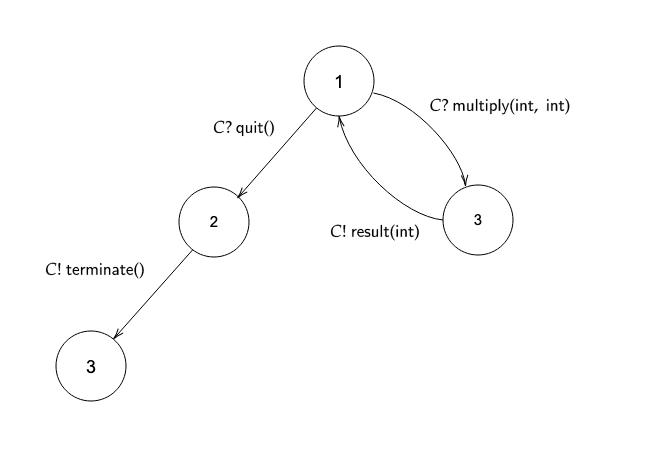
\includegraphics[scale=0.53]{scribble_fsm.png}
    \caption{CFSM for role S in Calculator Protocol}
    \label{scribble_fsm}
\end{figure}{}
We describe how the CFSMs can be used to generate code in an OOP programming language like Java for the different endpoints (roles) in the protocol. Each of the states in the CFSM is converted to a class with methods for each of the outgoing transitions from the current state, which carry out the necessary communication operations and return the next state. The user can chain calls to these methods to carry out the protocol, transitioning only between valid states until the final state is reached, which does not have any outgoing transitions. \\

In order to ensure the correctness of the implementation, every state must only be used once, which may require run-time checks. Implementations using the Scribble-generated APIs benefit from the correctness guarantees of MPST, ensuring that there are no communication errors and that the protocol is followed properly.\\

\section{Nested Protocols}
\subsection{Motivations}
The theory of session types has been extended in different directions in order to be able to become more expressive. Some advances have made it possible to annotate the protocol with logical assertions to define extra properties that the protocol should meet\cite{logicaassertions}. Other developments have made it possible to express protocols with parametrised roles\cite{parametrictypes} (expressing protocols where $n$ participants carry out particular roles), or to have greater control over how participants can join or leave a session through a dynamic multiparty session\cite{multirolesessiontypes}. \\

Demangeon et al.\cite{nestedprotocols} try to address a different challenge: protocols used in networking and in distributed systems are increasingly large. In many cases, they are highly modular, and often different protocols share the same structure. In order to better define and manage these protocols they extend the theory of session types to include nested protocols, which make it possible to define complex protocols using a simpler modular structure. Using this approach, protocols which have a similar structure can be grouped together under a single parametrised protocol, and complex protocols which might call other protocols can be expressed by making a call to those subprotocols. Moreover, different calls to the same subprotocol can be made with different parameters to achieve different behaviours. Their theory also allows subprotocols to bring in new participants by `inviting' them to participate. This can help simplify some protocols, as it allows you specify protocols where participants are brought in/contacted only if required.

\subsection{Session Calculus}
The theory they proposed is based on the idea of nesting protocols, where a parent protocol may define independent subprotocols and call them during its execution. Calls to a protocol can pass in different kinds of arguments as parameters such as values, roles from the parent protocol which will participate in the subprotocol and even other protocols which might be used during the call, similar to higher-order functions in functional programming.\\ 

Subprotocols are implemented as subsessions. The participant calling the protocol will create a new private session for its execution, and will send \textit{internal invitations} to all the roles in the parent protocol which will participate, and \textit{external invitations} to bring in new agents. In this way, only the roles which have a access to the subsession, so the other roles in the parent session will not be able to interfere with it. This model thus allows private interactions in a public session. The Scribble language described in Section \ref{Scribble} also allows subprotocols. However, as opposed to this theory, the roles participating in Scribble protocols have to be known statically, meaning that a call corresponds to inlining the subprotocol.\\

Calling subprotocols also abstract away their actual implementation, which means that the implementation of the subprotocol can be changed (e.g. to change how authentication is carried out or to improve the protocol's security) without changing the implementation of the parent protocol. Subprotocols also give a better separation between the different execution branches of the protocol, as different external participants can be invited only when required, reducing the complexity and utilisation of resources. For instance, in an HTTP-like protocol a proxy could have the choice of either returning a cached response directly or to initiate a \textit{Contact} protocol to involve the server and get the response. \\

\begin{figure}[h]
    \centering
    \begin{equation*}
    \centering
    \begin{array}{rrlcr}
        P,\ Q & ::= && \white & Processes \\[2.75pt]
             &   & 0 & \white & Nil\ Process  \\[2.75pt]
             & | & P\ |\ Q & \white & Parallel\ Composition  \\[2.75pt]
             & | & a(x).P & \white & Receive\ Ext.\ Invitation \\[2.75pt]
             & | & \overline{a}\langle s \rangle.P & \white & Send\ Ext.\ Invitation \\[2.75pt]
             & | & P\ +\ P & \white & Non-determinism\\[2.75pt]
             & | & k?[r, r]_{i \in I} \{l_i(x_i).P_i\}& \white & Branching \\[2.75pt]
             & | & k![r, r]l \langle v \rangle.P & \white & Selection \\[2.75pt]
             & | & (\nu\ u)\ P & \white & Scope\ Restriction\\[2.75pt] 
             & | & \texttt{new}\ s\ \texttt{on}\ k\ \texttt{with}\ (\widetilde{v})\&(\widetilde{a}\ \texttt{as}\ \widetilde{r}).P & \white & Subprotocol\ Call\\[2.75pt]
             & | & s \downarrow [r,\ r_1 : r_2](x).P & \white & Receive\ Internal\ Invitation\\[2.75pt]
             & | & s \uparrow [r,\ r_1 : r_2]\langle s \rangle.P & \white & Send\ Internal\ Invitation\\[2.75pt]
             & | & \mu X(x).P\langle v \rangle & \white  & Recursive\ Process \\[2.75pt]
             & | & X\langle v \rangle & \white  & Recursive\ Variable\\\\

        % M & ::= &&& Multiparty\ Session\\[2.75pt]
        % & | & p :: P\ & \white & Process\\[2.75pt]
        % & | & M\ |\ M\ & \white & Parallel\ Composition\\\\
        &&s,\ k,\ ... & \white & Session\ names\\[2.75pt]
        &&a,\ b,\ u,\ ... & \white & Shared\ channels\\[2.75pt]
        &&v & \white & Values\\
        &&r,\ r',\ ... & \white & Role\ Identifiers\\[2.75pt]
        &&x,\ y,\ z,\ ... & \white & Variables
        \end{array}
    \end{equation*}
    \caption{Processes in Session Calculus for Nested Protocols}
    \label{nested_session_calculus}
\end{figure}{}

Figure \ref{nested_session_calculus} shows the session calculus presented in the paper which includes the syntax for invitations and defining protocols. The calculus is based on the $pi$-calculus and shares a lot of the constructs of other existing session calculi\cite{logicaassertions}. Names are divided into two kinds: session channels, which handle all exchanges within a session, and shared channels, used to send and receive external invitations. 
\begin{itemize}
    \item Parallel composition, scope restriction and the nil process are defined as before.
    \item Recursion is also defined in a similar way as before, but it allows passing in a value to the recursive call which may be used when the recursive call is expanded. 
    \item $a(x).P$ and $\overline{a}\langle s \rangle.P$ are used for receiving and sending external invitations over the shared channel $a$.
    \item $P\ +\ P$ is the non-deterministic process. Execution can continue with either one of the two processes.
    \item $k?[r_1, r_2]_{i \in I} \{l_i(x_i).P_i\}$ is the branching operation from $r_1$ to $r_2$ with continuation $P_i$ in session $k$. $k![r_1, r_2]l \langle v \rangle.P$ is the selection operation, its dual primitive. 
    \item $s \downarrow [r,\ r_1 : r_2](x).P$ is the action for waiting for an internal invitation sent by $r$ to $r_1$ in order to play role $r_2$ in session $s$. 
    \item $s \uparrow [r,\ r_1 : r_2]\langle s \rangle.P$ is the action of sending an invitation from $r$ to $r_1$ in order to play role $r_2$ in session $s$.
    \item $\texttt{new}\ s\ \texttt{on}\ k\ \texttt{with}\ (\widetilde{v})\&(\widetilde{a}\ \texttt{as}\ \widetilde{r}).P$ is the operation for calling a subprotocol. Creates a new subsession $s$ within the parent session $k$, passing in arguments $\widetilde{v}$ and using shared channels $\widetilde{a}$ to send the external invitations.
\end{itemize}

\subsection{Session Types}
The paper also extends the syntax of session types to include the types for defining and calling subprotocols as well as sending and receiving invitations. The extended syntax for local and global types is shown in Figure \ref{nested_session_types}. They define kinds (types for types), including $\diamond$, which represents the protocol type, in order to formalize the definition of protocols. The definition of global types is essentially the same as before:
\begin{itemize}
    \item Termination, branching and recursion are almost the same as before. They also define the type for parallel composition.
    \item They introduce the construct $G_1\ \bigoplus^r\ G_2$ to represent located choice, where role $r$ can choose between two different branches. 
    \item $\texttt{let}\ \mathcal{P}\ =\ \lambda\widetilde{r}^1,\ \widetilde{y} \mapsto \texttt{new}\ \widetilde{r}^2.G\ \texttt{in}\ G'$ defines a subprotocol $\mathcal{P}$. The vector of roles $\widetilde{r}^1$ defines a set of roles that will be carried out by roles from the parent protocol which will be internally invited, whereas the vector $\widetilde{r}^2$ contains the set of roles which will be externally invited. The protocol also takes in vector of values $\widetilde{y}$.
    \item $r\ \texttt{calls}\ \mathcal{P}\langle \widetilde{r},\ \widetilde{y}\rangle.G$ is the subprotocol call carried out by role $r$, internally inviting roles $\widetilde{r}$ and passing in the values $\widetilde{y}$.
\end{itemize}{}

Similarly, the local session types are also very similar with the exception of the new constructs to handle invitations and protocol calls:
\begin{itemize}
    \item Termination, branching, selection and recursion are almost unchanged, and they introduce a type for parallel composition. 
    \item The construct $T_1\ \bigoplus^r\ T_2$ represents located choice.
    \item $\texttt{call}\ \mathcal{P}:G\ \texttt{with}\ (\widetilde{v}\ \texttt{as}\ \widetilde{y}:\widetilde{S})\&(\widetilde{r}^2).T$ is a call to the subprotocol $\mathcal{P}$, which has global type $G$, sending a vector of values $\widetilde{v}$ as arguments with sorts $\widetilde{S}$ and externally inviting the roles in $\widetilde{r}^2$ to participate in the subprotocol.
    \item Sending and accepting invitations for a role $r$ are handled by the $\texttt{req}\ \mathcal{P}[r]\langle \widetilde{v} \rangle\ \texttt{to}\ r.T$ and $\texttt{ent}\ \mathcal{P}[r]\langle \widetilde{v} \rangle\ \texttt{from}\ r.T$ constructors respectively.
\end{itemize}{}

\begin{figure}[h]
    \centering
    \begin{equation*}
    \centering
    \begin{array}{rrlr}
        Val & ::= & \texttt{int}\ |\ \texttt{bool}\ |\ \texttt{string} & Sorts\\\\
        K, S & ::= & Role\ |\ Val\ |\ \diamond\ |\ (K_1\ \times\ ...\ \times\ K_n) \longrightarrow K & Kinds\\\\
        
        \textsc{Global\ Types} & & &\\[3pt]
        G & ::= & \texttt{end} & Termination  \\[2.75pt]
             & | & \texttt{let}\ \mathcal{P}\ =\ \lambda\widetilde{r}^1,\ \widetilde{y} \mapsto \texttt{new}\ \widetilde{r}^2.G\ \texttt{in}\ G' & Subprotocol\ Def\\[2.75pt]
             & | & r\ \texttt{calls}\ \mathcal{P}\langle \widetilde{r},\ \widetilde{y}\rangle.G  & Subprotocol\ Call \\[2.75pt]
             & | & r_1 \longrightarrow r_2: \sum_{i \in I}\{l_i( S_i).G_i\} &  Branching \\[2.75pt]
             & | & G_1\ \bigoplus^r\ G_2   & Located Choice \\[2.75pt]
             & | & G_1\ |\ G_2 & Parallel\ Composition \\[2.75pt]
             & | & t & Type\ Variable \\[2.75pt]
             & | & \mu t.G & Recursive\ Type\\\\
             
        \textsc{Local Types} &&& \\[3pt]
        T & ::= & \texttt{end} &  Termination  \\[2.75pt]
          & | & \texttt{send}[r]!_{i \in I}\{ l_i(x_i: S_i).T_i\} & Selection \\[2.75pt]
          & | & \texttt{get}[r]?_{i \in I}\{l_i(x_i:S_i).T_i\} &  Branching \\[2.75pt] 
          & | & T_1\ \bigoplus \ T_2   & Located Choice \\[2.75pt]
          & | & T_1\ |\ T_2 & Parallel\ Composition \\[2.75pt]
          & | & \texttt{call}\ \mathcal{P}:G\ \texttt{with}\ (\widetilde{v}\ \texttt{as}\ \widetilde{y}:\widetilde{S})\&(\widetilde{r}^2).T &  Subprotocol Call \\[2.75pt]
          & | & \texttt{ent}\ \mathcal{P}[r]\langle \widetilde{v} \rangle\ \texttt{from}\ r.T &  Accept Invitation \\[2.75pt]
          & | & \texttt{req}\ \mathcal{P}[r]\langle \widetilde{v} \rangle\ \texttt{to}\ r.T &  Send Invitation \\[2.75pt]
          & | & t &  Type\ Variable \\[2.75pt]
          & | & \mu t.T &  Recursive\ Type
        
        \end{array}
    \end{equation*}
    \caption{Syntax of Session Types for Nested Protocols}
    \label{nested_session_types}
\end{figure}{}

As before, deriving the local types from the global type is done through the projection operation. It works very much in the same way as before, although now it becomes necessary to define a protocol environment to hold the types of the nested protocols, which gets updated by the $let\ in$ constructor.\\ 

Figure \ref{nested_session_projection} shows the definition of projection for the nested protocol definition and call. Projection on the remaining constructors is defined in the standard way. Projection of a protocol definition updates the environment with the protocol's global type and signature and continues recursively projecting the type. When projecting a nested protocol call onto a role $r^p$, there are multiple cases to consider:
\begin{itemize}
    \item if $r^p$ is the caller but does not participate itself in the subprotocol, the projection must only send out the internal invitations in parallel, as well as executing the projection of the continuation.
    \item if $r^p$ is the caller as well as a participant, then it must also send all the internal invitations to all the participating roles, but that includes itself, it must also accept its own invitation.
    \item if $r^p$ did not call the protocol but is a participant of the protocol, then it must simply accept the invitation, with the continuation being the projection of the continuation of the global type.
    \item otherwise, $r^p$ is neither a participant or the caller, so the projection is the projection of the continuation of the global type.
\end{itemize}

\begin{figure}[h]
    \centering
    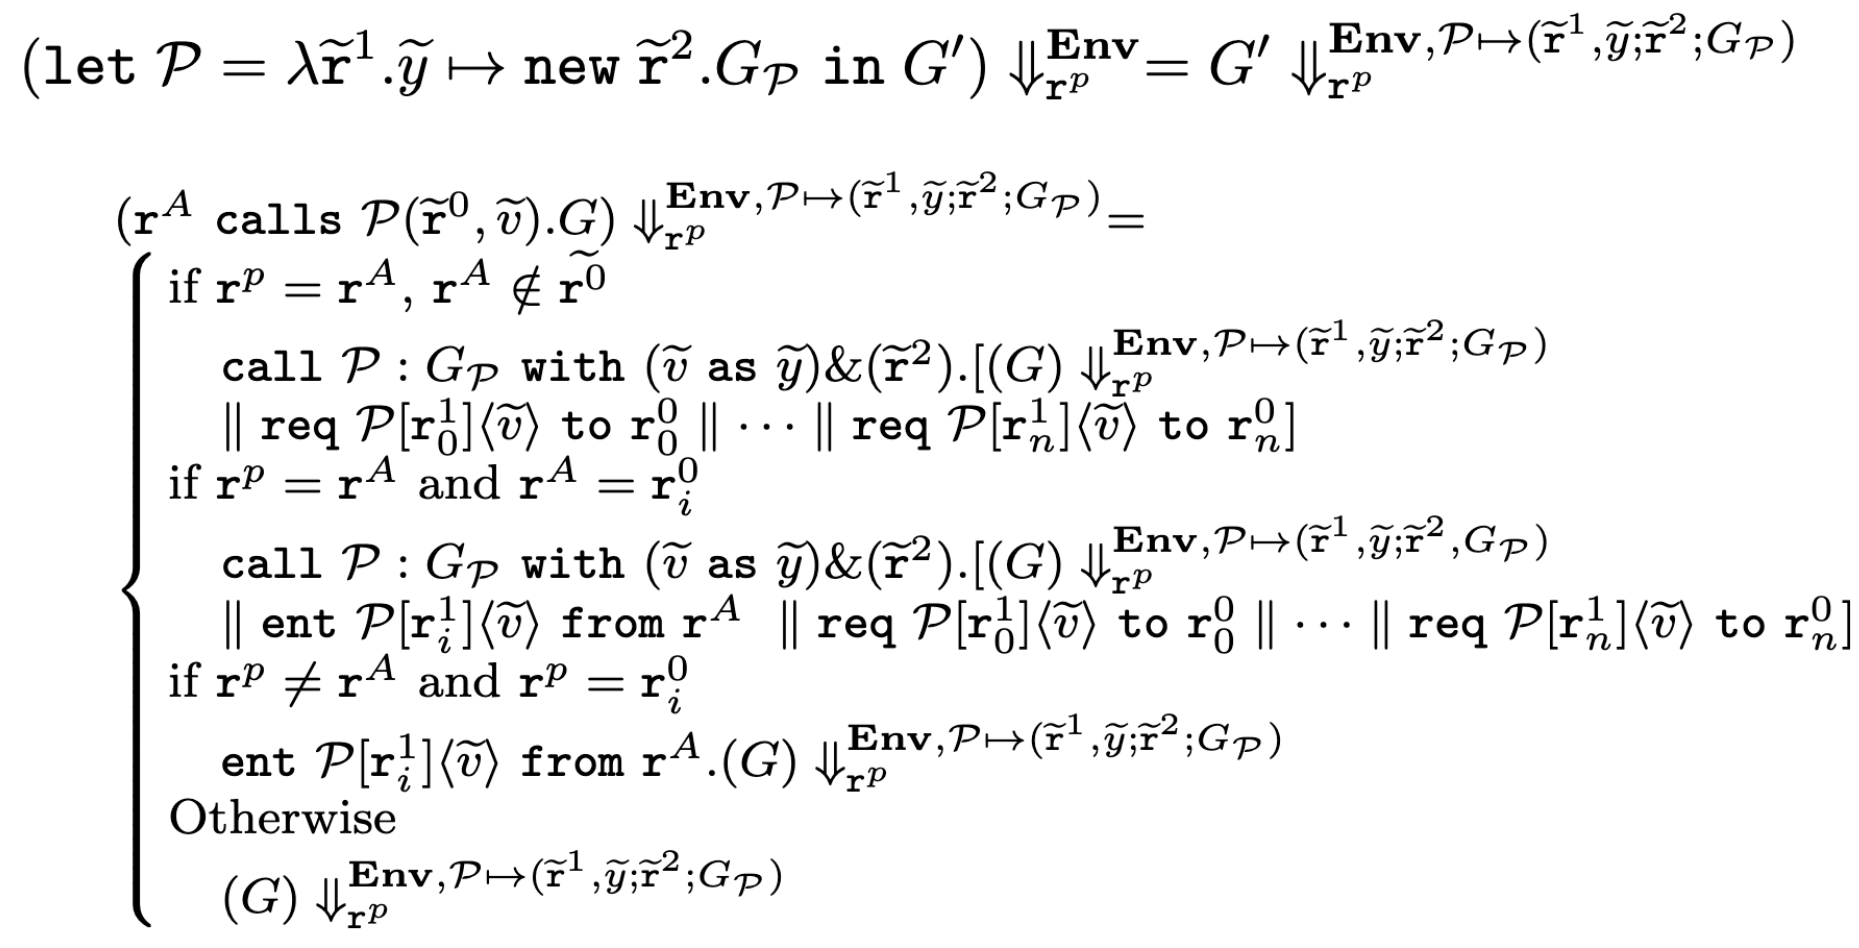
\includegraphics[scale=0.45]{nested_session_projection.png}
    \caption{Projection of Global Type in Nested Protocols\cite{nestedprotocols}}
    \label{nested_session_projection}
\end{figure}{}

\subsection{Returning Values from Subprotocols}
One limitation of the formulation expressed above is the inability of communication from a subsession back to the parent subsession. This means that it is impossible to express in a session type the relationship between a value calculated during a subsession and a value which a role might send after the nested protocol has ended. \\

For example, in the Client-Proxy-Server protocol described in Figure \ref{nested_session_example}, the value the server returns is $ans$, but that value cannot be seen outside of the $Contact$ subprotocol, so the proxy (middle) can only return $ans_0$ after completing the call to $Contact$. However, there are no guarantees that these two values are the same. The paper proposes some further extensions to the syntax of session types in order to make the protocol end by returning a value to the role which initiated the call in order to be able to capture be able to return information from the subprotocol. \\

Nevertheless, the current theory will suffice in most scenarios, as the kinds of the messages alone restrict what values can be sent, and it is up to the user's implementation to decide which value to send. Any value which satisfies this constraint can be considered a valid implementation of the protocol.
\begin{figure}[h]
    \centering
    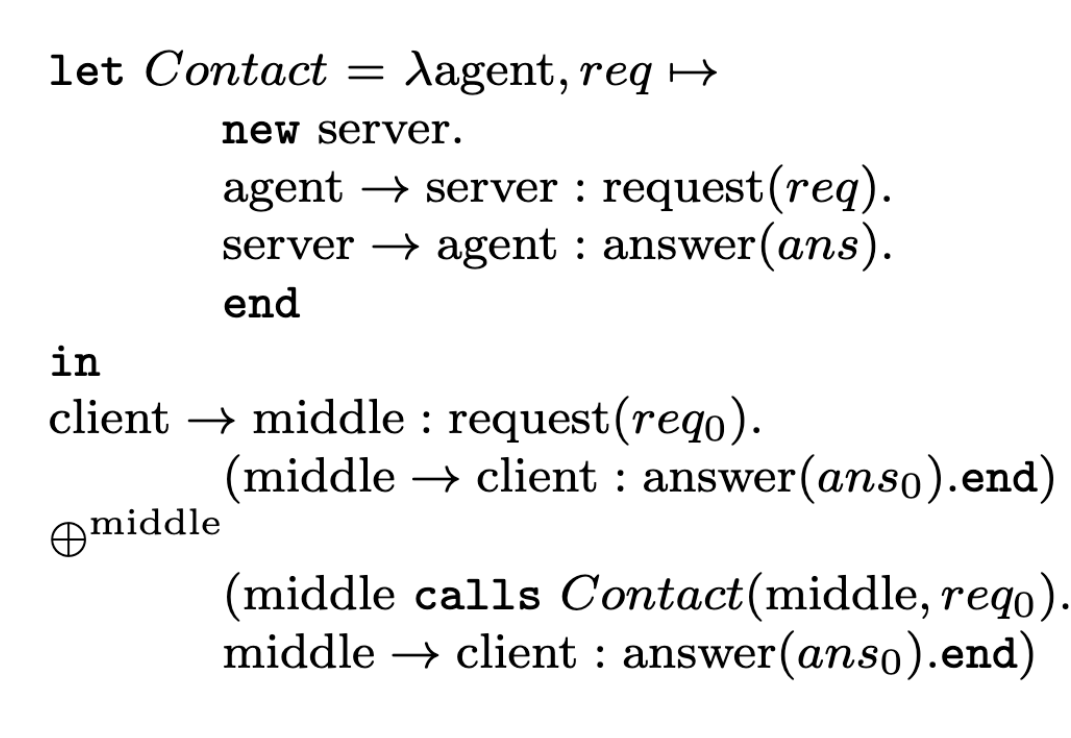
\includegraphics[scale=0.5]{nested_session_example.png}
    \caption{Example of Global Session Type for CPS Protocol\cite{nestedprotocols}\comment{nested protocols snippet}}
    \label{nested_session_example}
\end{figure}{}

% \subsection{Code Generation in Golang}
% Gois a popular industrial systems language.1One of its primary design features is first-classlanguage support for lightweight concurrency on multicore machines. Go offers easy spawningof parallel coroutines, calledgoroutines, that are transparently multiplexed over an underlyingset of system threads. Goroutines communicate and synchronize via message passing over typedchannels, designed to alleviate the difficulties of low-level mechanisms such as mutexes, conditionvariables and memory barriers commonly used in systems programming. As first-class objects, aninteresting andusefulfeature is the ability to passchannels over channels.Go is also well-established in distributed systems; e.g., it is the implementation language offrameworks such as Kubernetes, Docker and Jaeger. As the aforementioned concurrency features ofGo are specific to shared memory, a significant class of distributed programming in Go is conductedusing channel-based networking libraries via TCP, HTTP, etc. as transports. Developers appreciateGo since distributed programming in practice often involves local concurrency: goroutines andchannels are effective for dealing locally with the inherent asynchrony of distributed interactions
% For this project, the aim is to be able to generate a correct implementation of a protocol which uses nested protocols given a MPST-based specification. The target language for the framework to be developed is Go. Go is a popular programming language in industry. It has already been used to develop large projects like Docker and Kubernetes, and one of the reasons for its popularity is that it has inbuilt concurrency mechanisms. It has light-weight 

% In order for a global type to be well-formed, it must be projectable and well-kinded. Informally, well-kind which informally means that a mapping from all the identifiers in the global type to kinds can be found which 
%%%%%%%%%%%%%%%%%%%%%%%%%%%%%%%%%%%%

\chapter{API Generation using Scribble }
% TODO: Verify this after extending Scribble background
In this chapter we present a version of the Scribble protocol language as presented in \cite{scribble}, extended with constructs in order to be able to encode nested sessions. The code generation approach is different from the one previously discussed, as the code is generated directly from the session types. We describe the Scribble language extensions and the code generation approach to produce Golang APIs.

\section{Syntax Extensions} 

The Scribble syntax already has most of the constructs to encode the session types described in the nested sessions paper\cite{nestedprotocols}, but some of them are missing, like the internal choice session type. We have decided to focus on implementing functionality related to nested protocols, so we will not support internal choice. However, this should not be a great limitation, as the \texttt{choice} construct will suffice for most use cases.
\\

We also do not support the ability to send values when calling a nested protocol explicitly, but it in the protocol implementation we provide a means for the user to pass in values to subsessions by initialising the state of the different roles which will participate in the nested protocol.\\

The well-formedness property for protocols remains the same as before\cite{nestedprotocols}\cite{featherweight}. We say a protocol is well-formed if it is projectable, if the projection is defined for all the participants of that protocol. We incorporate the merging operator into the projection, which the original paper did not, extending the definition with the cases for invitations.

\subsection{Global Protocols}

We propose the following extensions to the scribble syntax for global protocols with nested protocols and subsessions:

\begin{itemize}
    \item $Module ::= N* P+$
    \item $N ::=\nested\ \protocol\ pro(\role\ A_1,\ ...,\ \role\ A_n;\ \scrnew\ \role B_1,\ ...,\ \role\ B_m)\ \{G\}$
    \item  $P ::=\nested\ \protocol\ pro(\role\ A_1,\ ...,\ \role\ A_n)\ \{G\}$
    \item $G ::= $
    
    $\quad\quad|\ N\ G $
    
    $\quad\quad|\ \choice\ \at\ A\ \{G_1\}\ \scror\ ...\ \scror\ \{G_n\}$

    $\quad\quad|\ a(S)\ \from\ A\ \scrto\ B;\ G$
    
    $\quad\quad|\ \rec\ t\ \{G\}$
    
    $\quad\quad|\ \continue\ t$
    
    $\quad\quad|\ \scrdo\ pro(A_1,\ ...\ ,\ A_n);\ G$

    $\quad\quad|\ A\ \calls\ pro(A_1,\ ...\ ,\ A_n);\ G$
\end{itemize}

A Scribble module can contain many top-level nested protocols, but it must contain at least one global protocol (with no dynamic roles), which can be used as the entry point for the computation.\\

Although nested protocols can be defined in any scope, for ease of parsing in the Scribble implementation and to provide more structured Scribble modules, we restrict where nested protocol can be declared. At the top-level, any nested protocols must be defined before the global protocol declarations, and within other protocols, they must be declared before any of the interactions. However, these restrictions do not impact the expressiveness of the implementation, as the order of the protocol declarations does not affect their scope.\\

We further explain the different modifications to the Scribble syntax:
\begin{itemize}
    \item The \texttt{nested} keyword can be used to define protocols with dynamic participants. Dynamic participants, are separated from the regular participants by a \texttt{new} keyword in the protocol declaration. However, dynamic protocols need not have dynamic participants, in which case the latter part of the declaration can be omitted. Like in the paper, nested protocols can be defined both at the top level and within other protocols. When a protocol is defined within another protocol, it restricts the scope where it can be used, much like defining a nested function in a programming language. We also allow shadowing of protocol names. If you redefine a protocol in an inner scope, then it will take override the previous definition in the current scope and all its subscopes.
    \item The \texttt{calls} construct introduces a subsession when a role calls a nested protocol. In a \texttt{calls} construct the dynamic participants of the nested protocol are omitted - it is only necessary to specify which existing roles which be participating, as the remaining roles will be dynamically created.
    \item We modify the semantics of \texttt{do} construct, which previously resulted in expanding the interactions of the called protocol, to instead create a subsession. It's semantics are equivalent to a \texttt{calls} construct, where the first partipant in the protocol is treated as the caller. While the \texttt{calls} construct deals can be used to call nested protocols, the \texttt{do} construct can only be used for global protocols. 
    \item The distinction between global and nested protocols is important, and needs to be verified to ensure that any protocol call used the correct construct. Moreover, protocol calls need to be verified to ensure that the call matches the signature of the protocol which is in scope, both for global and nested protocols.
\end{itemize}

Examples of these new features can be seen in Figure \ref{scribble-nested-global}.

\begin{figure}[h]
    \centering
    \lstset{language=Scribble}
    \begin{lstlisting}
    
    nested protocol NestedProtocol(role X; new role Y) {
        do GlobalProtocol(X, Y);
    }
    
    global protocol GlobalProtocol(role A, role B) {
        B calls NestedProtocol(A);
    }
        \end{lstlisting}
        \caption{Scribble syntax for nested protocols}
        \label{scribble-nested-global}
    \end{figure}{}

\subsection{Local Protocols}

We also had to modify the definition of projection of Scribble global types presented in \cite{featherweight} to include these new constructs. We therefore extend the syntax of Scribble local types with constructs for sending and receiving invitations following the session types presented in \cite{nestedprotocols}. 


\begin{itemize}
    \item $L ::=\scrlocal\ \protocol\ A@pro(\role A_1,\ ...,\ \role A_n;\ \scrnew\ \role B_1,\ ...,\ \role\ B_m)\ \{T\}$
    \item $T ::= $
    
    $\quad\quad|\ \choice\ \at\ A\ \{T_1\}\ \scror\ ...\ \scror\ \{T_n\}$

    $\quad\quad|\ a(S)\ \from\ B;\ T$

    $\quad\quad|\ a(S)\ \scrto\ B;\ T$
    
    $\quad\quad|\ \rec\ t\ \{T\}$
    
    $\quad\quad|\ \continue\ t$
    
    $\quad\quad|\ \invite(A_1,\ ...\ ,\ A_n)\ \scrto\ pro;\ T$
    
    $\quad\quad|\ \create(\role\ B_1,\ ...\ ,\role\ B_n)\ \scrin\ pro;\ T$

    $\quad\quad|\ \accept\ C@pro(A_1,\ ...\ ,\ A_n;\ \scrnew\ B_1,\ ...\ ,\ B_m)\ \from\ A;\ T$
\end{itemize}

After blurring the distinction between calling nested protocols and global protocols, we consider all local protocols to optionally have dynamic participants. We also expand the nested protocols so that all the protocol projections of a Scribble module are at the top level. Due to possible clashes between different protocols there may be a need to modify the protocol names to make them unique.

The constructs introduced here closely ressemble the session types presented in the nested protocols paper\cite{nestedprotocols}, and we briefly describe them here:

\begin{itemize}
    \item The sending of internal invitations is expressed by the \texttt{invite} construct, which specifies the roles which are going to participate, and the name of the protocol to which they are invited.
    \item Bringing new participants into the subsession through external invitations is done through the \texttt{create} statement, which specifies the dynamic roles of the protocol to be created. This can be omitted if there are no dynamic participants.
    \item Internal invitations are accepted through the \texttt{accept} construct, which contains information about the participant which sent the inviation, the local protocol which the role is going to be carrying out as well as all the other roles which will be participating as well.
\end{itemize}

Examples showcasing these new constructs can be seen in Figure \ref{scribble-nested-local}, which correspond to the projections of the protocols shown in Figure \ref{scribble-nested-global}:

% TODO: verify projection
\begin{figure}[h]
    \centering
    \lstset{language=Scribble}
    \begin{lstlisting}
    
    local protocol X@NestedProtocol(role X; new role Y) {
        invite(X, Y) to GlobalProtocol;
        accept A@GlobalProtocol(X, Y);
    }

    local protocol Y@NestedProtocol(role X; new role Y) {
        accept B@GlobalProtocol(X, Y);
    }
    
    local protocol A@GlobalProtocol(role A, role B) {
        accept X@NestedProtocol(A; new Y) from B;
    }

    local protocol B@GlobalProtocol(role A, role B) {
        invite(A) to NestedProtocol;
        create(role Y) in NestedProtocol;
    }
        \end{lstlisting}
        \caption{Scribble syntax for nested protocols}
        \label{scribble-nested-local}
    \end{figure}{}

\section{Projection}

The projection operation remains the same as defined in the Featherweight Scribble paper\cite{featherweight} for all constructs except the \texttt{choice} and \texttt{do}. For the projection of \texttt{choice} we extend the definition of the merging operation to incorporate invitations. The \texttt{do} construct is no longer expanded, it is treated as a call to a nested protocol where the participant which enacts the first role in the protocol is the one initiating the call with regards to projection.
\\

As in the original paper, projecting a global or nested protocol requires having an environment which keeps track of all the procols which are in scope. In the definition of projection below we assume that the given environment contains all the protocols which are in the scope of the protocol. We will describe a way of building such an environment later.

\subsection{Projection of Global Protocols}
We denote $\mathcal{P}(G)$ as the set of roles in protocol $G$. We define the projection of a Scribble nested protocol $P$ onto a role $A$ as follows: \\

If $A \in \{A_1,\ ...\ ,\ A_m,\ B_1,\ ...\ ,\ B_m\}$ then:

$(\nested\ \protocol\ P(\role\ A_1,\ ...\ ,\ \role\ A_n;\ \scrnew\ \role B_1,\ ...\ ,\ \role\ B_m)\ \{G\})\downarrow_A^{Env}\ =$

$\scrlocal\ \protocol\ A@P(\role A_1,\ ...\ ,\ \role A_n;\ \scrnew\ \role B_1,\ ...\ ,\ \role\ B_m)\ \{G \downarrow_A^{Env}\}$\\

Otherwise it is undefined. \\

Similarly for a Scribble global protocol. If $A \in \{A_1,\ ...\ ,\ A_m\}$ then:

$(\scrglobal\ \protocol\ P(\role\ A_1,\ ...\ ,\ \role\ A_n)\ \{G\})\downarrow_A^{Env}\ =$

$\scrlocal\ \protocol\ A@P(\role A_1,\ ...\ ,\ \role A_n)\ \{G \downarrow_A^{Env}\}$\\

Otherwise it is undefined.\\

We define the projection of a global protocol $G$ onto a role $A$ as follows:



\begin{figure}[h]
    \centering
    \begin{equation*}
    \centering
    \begin{array}{rcl}
        
        (a(S) & = &
        \begin{cases}
            \bigoplus_{i \in I}\ p'!l_i(S_i).(G_i \upharpoonright q) & \text{if}\ q\ =\ p\\
            \&_{i \in I}\ p?l_i(S_i).(G_i \upharpoonright q) & \text{if}\ q\ =\ p'\\
            G_{i_0} \upharpoonright q & \text{where}\ i_0 \in I,\ \text{if}\ q \notin \{p,\ p'\}\\
            & \text{and}\ \forall i,j \in I.\ G_i \upharpoonright q\ =\ G_j \upharpoonright q
        \end{cases}\\[33pt]
        (\mu t.G) \upharpoonright q & = & 
        \begin{cases}
            \mu t.(G \upharpoonright q) & \text{if}\ G \upharpoonright q \neq t\\
            \texttt{end} & otherwise
        \end{cases}\\[13pt]
        t \upharpoonright q & = & t\\[2.75pt]
        \texttt{end} \upharpoonright q & = & \texttt{end}\\[2.75pt]
        \end{array}
    \end{equation*}
    \caption{Projection of Global Types to Local Types}
    \label{MPST_projection}
\end{figure}{}


%%%%%%%%%%%%%%%%%%%%%%%%%%%%%%%%%%%%

%%%%%%%%%%%%%%%%%%%%%%%%%%%%%%%%%%%%
% \chapter{Contribution}

%%%%%%%%%%%%%%%%%%%%%%%%%%%%%%%%%%%%
% \chapter{Experimental Results}


%%%%%%%%%%%%%%%%%%%%%%%%%%%%%%%%%%%%
% \chapter{Conclusion}

\chapter{Notes}

\section{Issues}
\subsection{Code generation}
\begin{itemize}
    \item \textbf{Cyclic imports}:
    
    
    (Nested) protocols can call each other, having mutually recursive chains of calls. This means that the implementations of the roles for different protocols cannot be in different packages, as doing so would cause a cyclic import error, because the implementation of roles in one package would call functions in the other package, and vice versa.
    
    Similarly, the functionality for setting up a call to a nested protocol can't be in a separate package from the implementation of the roles for the protocols, as the setup will involve calling the implementation of the dynamic participants in the subprotocol, and some of the roles will rely on the setup function when preparing a call to the nested protocol. 
    
    States in callbacks may also depend on one another, as a call to a nested protocol will involve creating the state for that role in the nested protocol from the 
    
    \item \textbf{Waiting for dynamic participants}:
    
    Initially, it seemed that creating a \texttt{WaitGroup} to wait for all of the initial participants in the protocol to finish might be enough. However, after looking at several examples it became apparent that this was not the case. In nested protocols, dynamic participants could take much longer to complete all their interactions than the initial participants. This could happen for example when the initial participants carry out multiple calls to nested protocols, sending only a few messages at the start before finishing their roles. If there still remain interactions between dynamic participants (only), not waiting for all the dynamically started participants would end the protocol prematurely. 
    
    \item \textbf{Invitations}: We will consider invitations as a special kind of message sent between participants. Therefore, an invitation can be a valid message to determine which branch of a choice has been chosen as long as the invitation is a unique first message amongst all the branches of the choice - sending different invitations for the same protocol is also valid. From an implementation perspective, invitations are messages containing a struct with the channels that the participant will need to communicate with the other participants in the nested protocol. This set of channels will be fresh in order to guarantee a separation between the parent and child sessions.

    Roles in both global and nested protocols will have a separate set of channels stored in a struct which can be used to send and receive invitations to/from other participants in the same protocol. We chose to keep these channels separate from the other channels used to communicate with other participants because they are used to spend these special kinds of messages. However, this meant that the invitation channels' struct also had to include channels to send the invitation channels struct that the participant will use to send invitations in the nested protocol. Therefore, at the implementation level, our invitations consist of two messages, one for struct containing the channels the role will use to communicate with other participants and another one the struct containing the channels the role will use to send and receive invitations.
    
    Sent asynchronously. 
    Link to well-formed choice over synchronous channels, and allowing processes to proceed as soon as possible.
    
    \item \textbf{Well-formed choice}: In order for a choice to be well-formed, all roles in the choice must receive a distinct/unique first message from an enabled participant. This choice message must be sent over a dedicated channel used only for this choice. As discussed previously, invitations are sent asynchronously. If there was a single channel to send \texttt{Msg2()} between \texttt{A} and \texttt{B}, then \texttt{B}, who doesn't participate in \texttt{NestedProto}, will be able to continue sending \texttt{Msg2()} after it sends the invitations for \texttt{NestedProto}. This means that there will be a race as to which message \texttt{A} will receive first, because \texttt{A} would be waiting to receive either the invitation for \texttt{NestedProto} or \texttt{Msg2()} \textit{on the same channel} which \texttt{B} used to send \texttt{Msg2()} in the first branch. If \texttt{Msg2()} were received first, then the protocol would be stuck in a deadlock, because \texttt{A} would mistakenly identify the second branch as the branch which \texttt{B} chose. Therefore, \texttt{A} would be stuck waiting for a message from \texttt{B} which would never come, since \texttt{B} would be waiting for \texttt{Msg3()} from \texttt{A}.
    
    Otherwise, if the channel used to receive the choice message is the same as a channel used to send a message in some branch, there might be a deadlock, as the non-choice message might be sent and received before the actual choice message for a different branch was received. This would cause the participant to think wrongly identify the execution branch which was chosen. For example, in Figure \ref{deadlock} if there weren't separate channels for Msg2() in the first branch and Msg2() in the the second branch then if channels were asynchronous.
    
\begin{figure}[h]
\centering
\lstset{language=Scribble}
\begin{lstlisting}

nested protocol NestedProto(role X; new role Y) {
    [...]
}

global protocol Deadlock(role A, role B) {
    choice at B {
        B calls NestedProto(A);
        Msg2() from B to A;
        Msg3() from A to B;
    } or {
        Msg2() from B to A;
        Msg4() from B to A;
    }
}

local protocol Deadlock_A(self A, role B) {
    choice at B {
        accept X from B in NestedProto_X(self; new Y);
        Msg2() from B;
        Msg3() to B;
    } or {
        Msg2() from B;
        Msg4() from B;
    }
}

local protocol Deadlock_B(role A, self B) {
    choice at self {
        invite(A as X) in NestedProto;
        create(role Y) in NestedProto;
        Msg2() to A;
        Msg3() from A;
    } or {
        Msg2() to A;
        Msg4() to A;
    }
}

local protocol NestedProto_X(self X, role Y) {
    [...]
}
    \end{lstlisting}
    \caption{Choice ambiguity}
    \label{deadlock}
\end{figure}{}

    \item \textbf{Code gen design choices:}
    
    - Synchronous channels
    
    - Always send invitations over channels - unifority and single setup() function which can be called by different participants from different protocols
    
    - (Provisional) Callbacks using interfaces (structs which maintain state). Nested role may return result to caller function - this \textbf{will} \textbf{probably} be \textbf{removed}.
    
    - Probably don't allow protocols which don't have at least two participants??
    
    TODO: More elaborate examples and translation scheme from scribble to go. Possibly formalize Scribble projection as well.
    
    Possible two passes - one for channels and one for code generation
    
    Setup 
    
    \item \textbf{Code Gen} - name clashes
    Eg. consider when a nested and not nested protocol are defined at the top level. They are both "different" since one is called through do and the other through calls, and only one of them is a "nested" protocol. Handle through prefixing (eg. nested\_<proto>).
    
    \item \textbf{Scribble language extension} - design
    
    \textbf{Global Types}
    \begin{itemize}
        \item Allow nested protocols to be defined at the top level as well as nested within other global and nested protocols, before any of the protocol's interactions. However, restrict the order of the declarations. All nested protocols at the top level have to be defined before the global protocols. This doesn't affect the expressiveness of the language, it is just a structural limitation which simplified parsing. 
        \item Use "nested protocol" header to define a nested protocol
        \item Split the roles in a nested protocol's role declaration into two to distinguish dynamic from non-dynamic participants 
        \item Add new syntax for calling nested protocols: <role> calls <proto>(R1, ..., RN);
        This was to ensure that this new construct did not clash with the existing "do <proto>" construct which was used to call other global protocols. Each of the two constructs can be used to call nested/global protocols, but trying to call a nested protocol with 'do' or a global protocol with 'nested' would be invalid. However, at an implementation level, both are treated in the same way.
        \item Scopes
        
        Nested protocols introduce the notion of scopes to Scribble's protocol language. Before, everything was defined at the top level, so there was a single scope where protocols could be defined. However, nested protocols can be defined inside other protocols as well as at the top level, so it is important to ensure that protocols can only call protocols which are in scope. Much like functions in some programming languages, a protocol defines its own scope. All protocols within one scope are visible to one another, meaning that it is possible to define mutually recursive protocols. 
        
        Allowing scope definition can result in cases whose behaviour might not be very intuitive. If you define a nested protocol with the same name as the parent, any reference in the parent protocol's interactions to that name with call the nested protocol, not itself, because it shadows previous definition.
        
        \item Nested protocols, like global protocols must have at least two participants. Global protocols can only have 'static' participants, they cannot have dynamic participants. On the other hand nested protocols can have zero or more dynamic participants, but they must always have at least one non-dynamic participant. 
        
        Allowing a nested protocol to not have any dynamic participants does not impact the implementation in any way and allows greater flexibility when defining protocols. A nested protocol without dynamic participants is essentially the same as a global protocol, except that it's possible to define it inside other protocols, thereby restricting the scope from which it can be called.
        
        The restriction of having at least one (active) role which is not dynamic ensures that the protocol it is always possible for information to reach all the participants in a protocol. Allowing protocols made up of only dynamic participants means that a set of new participants would be brought together and they would perform a series of interactions and then leave without any of the roles in the calling scope communicating with them. This means that any information transferred during such a protocol cannot reach any of the participants in the calling scope, so the information from the exchanges in such a protocol is essentially lost. With the restriction in place, it would always be possible for a role which participated in a protocol call to transmit relevant information to other participants through further interactions with them.
    \end{itemize}
    
    \item \textbf{Parsing} - Extending Scribble parser
    Existing parser provided a wide array of options (although not all of them were implemented). (\textbf{TODO}: More detail about designing Scribble syntax for nested protocols).
    
    Scribble module design:
    \begin{itemize}
        \item module declaration
        \item type declarations
        \item nested protocol declarations - allow top-level nested protocol declarations to be able to define protocols which are in scope for all other nested/global protocols. They were grouped at together at the beginning of the file, as it simplified parsing.
        \item global protocol declarations
    \end{itemize}
    
    Scribble global type allows nested protocol definitions inside global and nested protocols.
    
    The naive implementation of the file structure defined above resulted in shift-reduce conflicts in the parser.
    Originally nested protocol definitions simply had "nested protocol" keywords in their header instead of "global protocol". However, in the parser, protocol definitions in the parser could also optionally have protocol options before the protocol header (eg. \textbf{aux explicit} global protocol X(...) \{...\}). Because the aim was to preserve as much of the existing syntax intact, the protocol options were also added to nested protocol declarations. This was a problem, as the parser could not distinguish the boundary between nested and global protocol declarations at the top level if the declarations included the protocol options. In order to overcome this issue three approaches were considered:
    \begin{itemize}
        \item Drop the protocol options in nested protocol declarations altogether - protocol options were not implemented yet for global protocols, and they were not necessary for the initial imp implementation of nested protocols. 
        \item Move the nested keyword before the protocol options in the declaration, thereby disambiguating between both kinds of declarations. 
        \item Add an explicit delimiter (\textbf{TODO: Decide on delimiter here}) between the nested and global protocol declarations at the top level.
    \end{itemize}
    
    AST for nested protocols was the same as as for global protocols, which meant that a lot of the exisiting implementation could be mimicked or used.
    
    \item \textbf{Protocol validation}
    
    Existing Scribble implementation allows defining multiple protocols in one module, when generating code the interactions of protocol which is being implemented will be expanded in order to remove all calls to other protocols. However in nested protocols, in order to mainitain a more modularized approach, interactions within a protocol are self-contained and implemented as a separate sub-session. This means that this process of expanding of the interactions was not needed. All that was required was to verify that all calls to nested/global protocols across all protcols were valid. This involved checking that:
    \begin{itemize}
        \item A call to a nested protocol
        
    \end{itemize}
    \textbf{TODO: Check for unused roles}
    \textbf{TODO: Mutually recursive protocol cycles}
    
    \item \textbf{Projection}
    Checking consistent choice: Any of the roles involved in a call are viable candidates to be the first receiver of the choice.

    blajodfhlkasjhfkajsdbflaksjdb
    fdsakjfhalsdk 
    \textbf{TODO: Verify - technically, the first message will always be for the role who will be the first participant in the protocol. Is it fine to consider all of them as a single unit, or should it just be the first one?}
\end{itemize}{}

%% bibliography
\bibliographystyle{acm}
% \nocite{*}
\bibliography{interimbib}

\end{document}